%\documentclass[12pt]{article}

%\usepackage{graphicx}
%\usepackage{caption}

%\begin{document}

%--------------------------------------------------------------------------------------------------------------------  
%--------------------------------------------------------------------------------------------------------------------

  \subsection{Hardware}  

  \newpage

%--------------------------------------------------------------------------------------------------------------------  
%--------------------------------------------------------------------------------------------------------------------

  \subsubsection{Diagrama de bloques (hardware)}

\begin{figure}[h!]
 \centering
 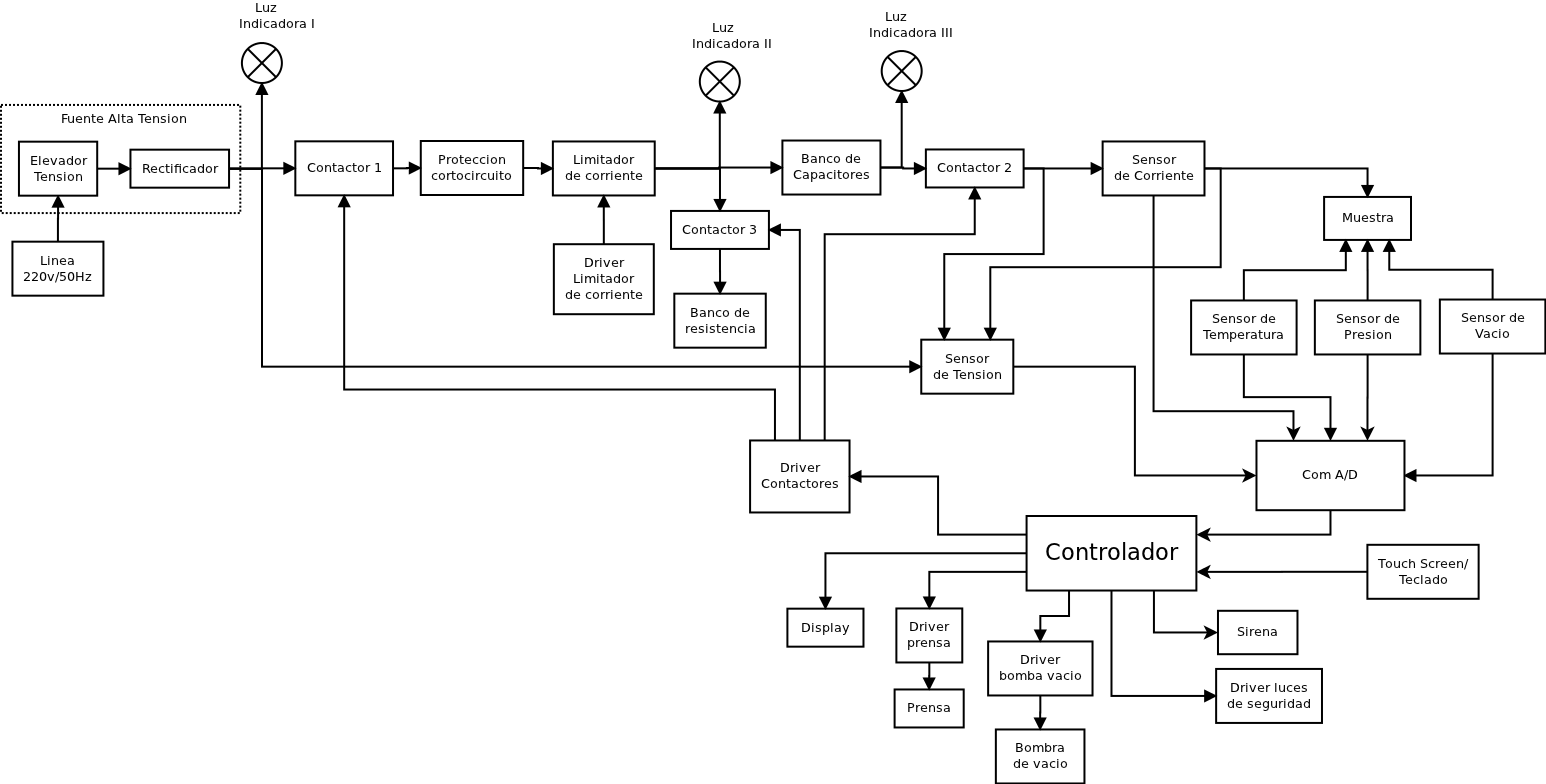
\includegraphics[height=330px, angle=90]{../../Documentacion/Diagramas/diagramaBloquesMacro.png}
 \caption{Diagrama en bloques general de la solución propuesta}
\end{figure}

%Otra versión del diagrama en bloques
% \begin{figure}[h!]
%  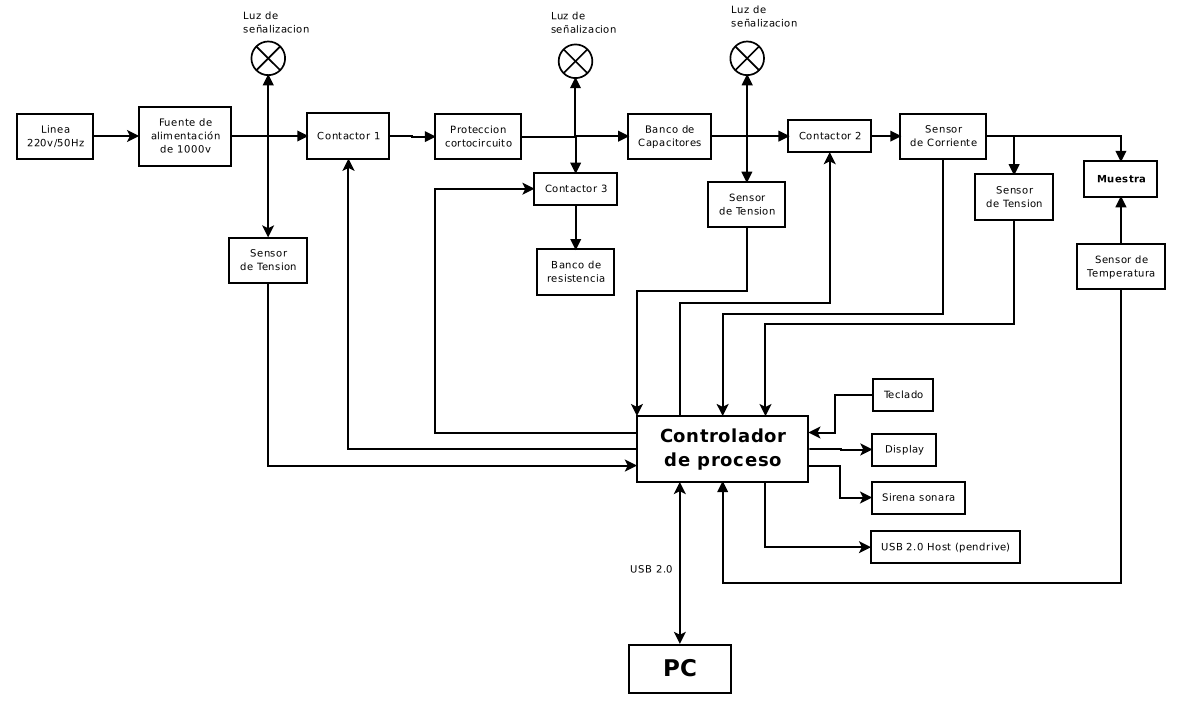
\includegraphics[width=500px]{../../../Documentacion/Diagramas/diagramaBloquesEspecificaciones.png}
%  % diagramaBloquesEspecificaciones.png: 1183x705 pixel, 96dpi, 31.30x18.65 cm, bb=0 0 887 529
%  \caption{Diagrama en bloques del proceso de sinterizado}
%  \label{fig:2}
% \end{figure}


  \newpage

%--------------------------------------------------------------------------------------------------------------------  
%--------------------------------------------------------------------------------------------------------------------

  \subsubsection{Detalles de selección y calculo de los elementos circuitales de cada bloque}  

  \newpage


%--------------------------------------------------------------------------------------------------------------------  
%--------------------------------------------------------------------------------------------------------------------

  \subsubsection{Plan de pruebas de cada modulo}  

  \newpage


%--------------------------------------------------------------------------------------------------------------------  
%--------------------------------------------------------------------------------------------------------------------

  \subsection{Software}  

  \newpage


%--------------------------------------------------------------------------------------------------------------------  
%--------------------------------------------------------------------------------------------------------------------

  \subsubsection{Diagrama de estados, procesos y flujogramas}  

  \newpage



%--------------------------------------------------------------------------------------------------------------------  
%--------------------------------------------------------------------------------------------------------------------

  \subsubsection{Análisis de complejidad (Mc.Cabe o Hasltead )}  

  \newpage



%--------------------------------------------------------------------------------------------------------------------  
%--------------------------------------------------------------------------------------------------------------------

  \subsubsection{Descripción de subrutinas}  

  \newpage



%--------------------------------------------------------------------------------------------------------------------  
%--------------------------------------------------------------------------------------------------------------------

  \subsubsection{Listados comentados del código }  

  \newpage


%--------------------------------------------------------------------------------------------------------------------  
%--------------------------------------------------------------------------------------------------------------------

  \subsubsection{Plan de prueba de módulos y de depuración de software}  

  \newpage

%--------------------------------------------------------------------------------------------------------------------  
%--------------------------------------------------------------------------------------------------------------------
%\end{document}
